\documentclass[../presentation.tex]{subfiles} % Parent file
\graphicspath{{\subfix{../images/}}} % Images path

\usetikzlibrary{positioning,3d}

\begin{document}

\section{Classification}

\begin{frame}
    
    \frametitle{Custom CNN Architecture}

        \begin{tikzpicture}[scale=0.6, 3d view={120}{20}]

            % Input layer (128x128x3)
            \draw[fill=cyan] (0, 0, 0) -- (0, 0, 4) -- (0, 5, 4) -- (0, 5, 0) -- cycle;
            \node[up right, rotate=43] at (0, 0, 7) {\scriptsize Input 128x128x3};

            % Convolutional layer 1 (kernel 9x9, 96 channels, stride 4)
            \draw[fill=orange] (1.3, 0, 0) -- (1.3, 0, 3) -- (1.3, 3, 3) -- (1.3, 3, 0) -- cycle;
            \draw[fill=orange] (1.3, 0, 0) -- (1.3, 0, 3) -- (1.6, 0, 3) -- (1.6, 0, 0) -- cycle;
            \draw[fill=orange] (1.3, 3, 0) -- (1.3, 3, 3) -- (1.6, 3, 3) -- (1.6, 3, 0) -- cycle;
            \draw[fill=orange] (1.6, 0, 0) -- (1.6, 0, 3) -- (1.6, 3, 3) -- (1.6, 3, 0) -- cycle;
            \draw[fill=orange] (1.3, 0, 3) -- (1.3, 3, 3) -- (1.6, 3, 3) -- (1.6, 0, 3) -- cycle;
            \node[up right, rotate=43] at (1.3, 0, 7) {\scriptsize Conv 9x9, stride 4};
            \node[up right, rotate=43] at (1.3, 3, -3) {\scriptsize 96 channels};

            % Batch normalization
            \coordinate (A) at (2, 0, 0);
            \coordinate (B) at (2, 0, 3);
            \draw[red, dashed] (A) -- (B) -- cycle;
            \node[up right, rotate=43] at (2, 0, 7) {\scriptsize Batch Normalization};

            % Max pooling
            \coordinate (A) at (2.5, 0, 0);
            \coordinate (B) at (2.5, 0, 3);
            \draw[blue] (A) -- (B) -- cycle;
            \node[up right, rotate=43] at (2.5, 0, 7) {\scriptsize Max pooling};

            % Convolutional layer 2 (kernel 5x5, 256 channels, stride 1)
            \draw[fill=orange] (3.3, 0, 0) -- (3.3, 0, 2.5) -- (3.3, 2, 2.5) -- (3.3, 2, 0) -- cycle;
            \draw[fill=orange] (3.3, 0, 0) -- (3.3, 0, 2.5) -- (4, 0, 2.5) -- (4, 0, 0) -- cycle;
            \draw[fill=orange] (3.3, 2, 0) -- (3.3, 2, 2.5) -- (4, 2, 2.5) -- (4, 2, 0) -- cycle;
            \draw[fill=orange] (4, 0, 0) -- (4, 0, 2.5) -- (4, 2, 2.5) -- (4, 2, 0) -- cycle;
            \draw[fill=orange] (3.3, 0, 2.5) -- (3.3, 2, 2.5) -- (4, 2, 2.5) -- (4, 0, 2.5) -- cycle;
            \node[up right, rotate=43] at (3.3, 0, 7) {\scriptsize Conv 5x5, stride 1};
            \node[up right, rotate=43] at (3.3, 2, -3) {\scriptsize 256 channels};

            % Batch normalization
            \coordinate (A) at (4.4, 0, 0);
            \coordinate (B) at (4.4, 0, 2.5);
            \draw[red, dashed] (A) -- (B) -- cycle;
            \node[up right, rotate=43] at (4.4, 0, 7) {\scriptsize Batch Normalization};

            % Max pooling
            \coordinate (A) at (4.9, 0, 0);
            \coordinate (B) at (4.9, 0, 2.5);
            \draw[blue] (A) -- (B) -- cycle;
            \node[up right, rotate=43] at (4.9, 0, 7) {\scriptsize Max pooling};

            % Convolutional layer 3 (kernel 3x3, 384 channels, stride 1)
            \draw[fill=orange] (5.7, 0, 0) -- (5.7, 0, 2) -- (5.7, 1, 2) -- (5.7, 1, 0) -- cycle;
            \draw[fill=orange] (5.7, 0, 0) -- (5.7, 0, 2) -- (6.8, 0, 2) -- (6.8, 0, 0) -- cycle;
            \draw[fill=orange] (5.7, 1, 0) -- (5.7, 1, 2) -- (6.8, 1, 2) -- (6.8, 1, 0) -- cycle;
            \draw[fill=orange] (6.8, 0, 0) -- (6.8, 0, 2) -- (6.8, 1, 2) -- (6.8, 1, 0) -- cycle;
            \draw[fill=orange] (5.7, 0, 2) -- (5.7, 1, 2) -- (6.8, 1, 2) -- (6.8, 0, 2) -- cycle;
            \node[up right, rotate=43] at (5.7, 0, 7) {\scriptsize Conv 3x3, stride 1};
            \node[up right, rotate=43] at (5.7, 1, -3) {\scriptsize 384 channels};

            % Batch normalization
            \coordinate (A) at (7.2, 0, 0);
            \coordinate (B) at (7.2, 0, 2);
            \draw[red, dashed] (A) -- (B) -- cycle;
            \node[up right, rotate=43] at (7.2, 0, 7) {\scriptsize Batch Normalization};

            % Convolutional layer 4 (kernel 3x3, 256 channels, stride 1)
            \draw[fill=orange] (8, 0, 0) -- (8, 0, 2) -- (8, 1, 2) -- (8, 1, 0) -- cycle;
            \draw[fill=orange] (8, 0, 0) -- (8, 0, 2) -- (8.7, 0, 2) -- (8.7, 0, 0) -- cycle;
            \draw[fill=orange] (8, 1, 0) -- (8, 1, 2) -- (8.7, 1, 2) -- (8.7, 1, 0) -- cycle;
            \draw[fill=orange] (8.7, 0, 0) -- (8.7, 0, 2) -- (8.7, 1, 2) -- (8.7, 1, 0) -- cycle;
            \draw[fill=orange] (8, 0, 2) -- (8, 1, 2) -- (8.7, 1, 2) -- (8.7, 0, 2) -- cycle;
            \node[up right, rotate=43] at (8, 0, 7) {\scriptsize Conv 3x3, stride 1};
            \node[up right, rotate=43] at (8, 1, -3) {\scriptsize 256 channels};

            % Batch normalization
            \coordinate (A) at (9.1, 0, 0);
            \coordinate (B) at (9.1, 0, 2);
            \draw[red, dashed] (A) -- (B) -- cycle;
            \node[up right, rotate=43] at (9.1, 0, 7) {\scriptsize Batch Normalization};

            % Max pooling
            \coordinate (A) at (9.6, 0, 0);
            \coordinate (B) at (9.6, 0, 2);
            \draw[blue] (A) -- (B) -- cycle;
            \node[up right, rotate=43] at (9.6, 0, 7) {\scriptsize Max pooling};

            % Fully connected layer 1 (1024 -> 512 features)
            \draw[fill=green] (10.4, -0.3, 0) -- (10.7, -0.3, 0) -- (10.7, 5, 0) -- (10.4, 5, 0) -- cycle;
            \node[up right, rotate=43] at (10.9, 0, 7) {\scriptsize Fully connected 1024 -> 512};

            % Dropout
            \coordinate (A) at (11.1, -0.3, 0);
            \coordinate (B) at (11.1, 5, 0);
            \draw[yellow, dashed] (A) -- (B) -- cycle;
            \node[up right, rotate=43] at (11.5, 0, 5) {\scriptsize Dropout};

            % Fully connected layer 2 (512 -> 128 features)
            \draw[fill=green] (11.8, -0.3, 0) -- (12.1, -0.3, 0) -- (12.1, 3.5, 0) -- (11.8, 3.5, 0) -- cycle;
            \node[up right, rotate=43] at (12.3, 0, 7) {\scriptsize Fully connected 512 -> 128};

            % Dropout
            \coordinate (A) at (12.5, -0.3, 0);
            \coordinate (B) at (12.5, 3.5, 0);
            \draw[yellow, dashed] (A) -- (B) -- cycle;
            \node[up right, rotate=43] at (12.9, 0, 5) {\scriptsize Dropout};

            % Output layer (128 features -> 4 classes)
            \draw[fill=blue] (13.2, -0.3, 0) -- (13.5, -0.3, 0) -- (13.5, 2, 0) -- (13.2, 2, 0) -- cycle;
            \node[up right, rotate=43] at (13.8, 0, 5) {\scriptsize Output 128 -> 4};
            
            \end{tikzpicture}

\end{frame}

\begin{frame}
    
    \frametitle{Training Details}

    Training parameters:
    \vspace{0.2cm}
    \begin{itemize}
        \item \textbf{Epochs}: $50$
        \item \textbf{Batch size}: $64$
        \item \textbf{Learning rate}: $1\times10^{-4}$
        \item \textbf{Optimizer}: Adam (weight decay $1\times10^{-5}$)
        \item \textbf{Scheduler}: stepLR (step size 10, gamma 0.5)
        \item \textbf{Loss function}: Cross-entropy
        \item \textbf{Activation function}: Mish
        \item \textbf{Dropout rate}: $0.4$
        \item \textbf{Image size}: $128\times128$
    \end{itemize}

\end{frame}

\begin{frame}
    
    \frametitle{Training Loss and Accuracy}

    \begin{center}
        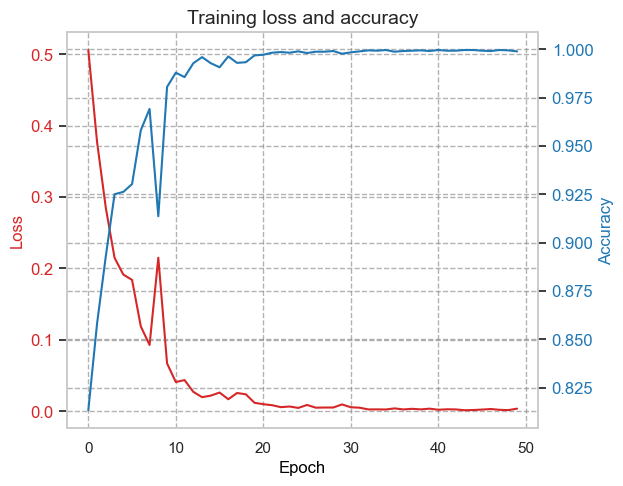
\includegraphics[width=0.65\textwidth]{loss-accuracy_customCNN.png}
    \end{center}

    \small{
    \begin{cbox}
        \begin{itemize}
            \item Final training loss: $3.6\times10^{-3}$
            \item Final training accuracy: $99.9\%$
        \end{itemize}
    \end{cbox}
    }

\end{frame}

\begin{frame}
    
    \frametitle{Confidence and Test Accuracy}

    \begin{center}
        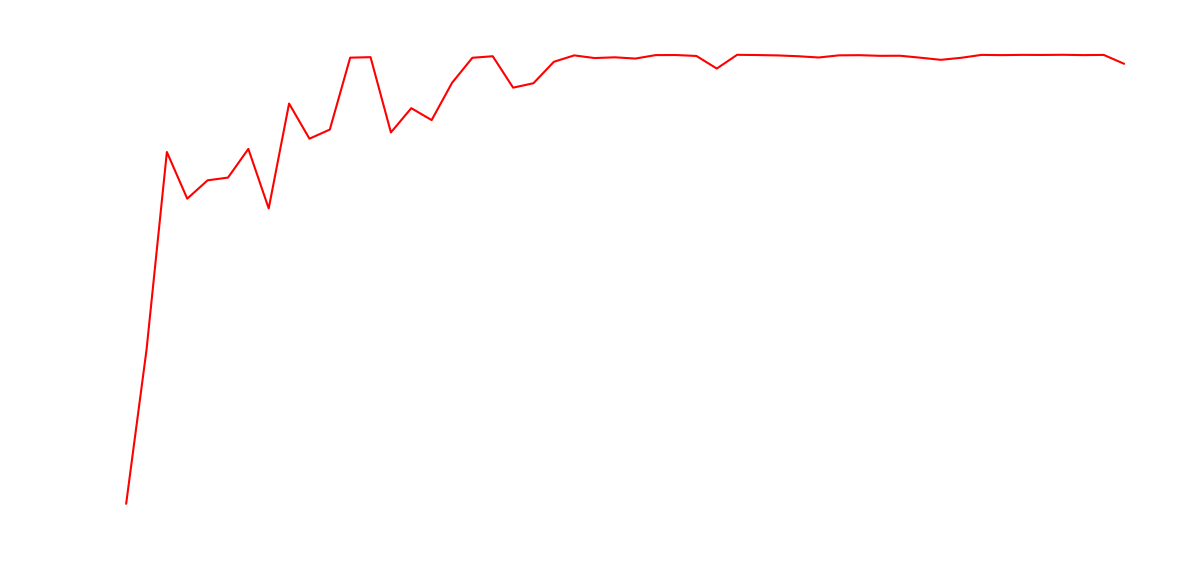
\includegraphics[width=0.65\textwidth]{confidence_customCNN.png}
    \end{center}

    \small{
    \begin{cbox}
        \begin{itemize}
            \item Final training confidence: $99.9\%$
            \item Final test confidence: $99.9\%$
            \item \red{Final test accuracy: $99\%$}
        \end{itemize}
    \end{cbox}
    }

\end{frame}

\end{document}